\documentclass[10pt]{beamer}

\newcommand{\lectnum}{L09}
\newcommand{\lecttitle}{Probabilistic Graphical Models}

\usepackage{amsmath, amssymb, graphicx}
\usepackage[]{algorithm2e}
\usepackage{pdfpages}
\usepackage[british]{babel}

\hypersetup{colorlinks,linkcolor=,urlcolor=blue}
\newenvironment{titledslide}[1]{\begin{frame}\frametitle{#1}}{\end{frame}}

\mode<presentation>{\setbeamercovered{transparent}}

\setbeamertemplate{sidebar right}{}
\setbeamertemplate{footline}{%
\hfill\usebeamertemplate***{navigation symbols}
\hspace{0.4cm}\lectnum: \insertframenumber{}/\inserttotalframenumber \hspace*{0.4cm}}

\author{James Cussens}

\title{COMS30035, Machine learning:\\ \vspace{5pt} \lecttitle}

\institute{School of Computer Science\\University of Bristol}

\begin{document}
%%%%%%%%%%%%%%%%%%%%%%%%%%%%%%%%%%%%%%%%%%%%%%%%%%%%%%%%%%%%%%%%%%%%%%

\begin{frame}
  \titlepage
\end{frame}

%%%%%%%%%%%%%%%%%%%%%%%%%%%%%%%%%%%%%%%%%%%%%%%%%%%%%%%%%%%%%%%%%%%%%%


\usetikzlibrary{bayesnet}
%\tikzstyle{const} = [circle, fill=white, minimum size=5pt, inner
%sep=0pt, node distance=0.4]
\tikzstyle{const} = [circle, fill=black, minimum size=3pt, inner
sep=0pt, node distance=1]

\newcommand{\ci}{\ensuremath{\perp}}
\newcommand{\params}{\ensuremath{\mathbf{w}}}
\newcommand{\dualparams}{\ensuremath{\mathbf{a}}}
\newcommand{\designm}{\ensuremath{{\bm \Phi}}}
\newcommand{\xvec}{\ensuremath{\mathbf{x}}}
\newcommand{\xvecn}{\ensuremath{\mathbf{x}_{n}}}
\newcommand{\feat}{\ensuremath{\phi}}
\newcommand{\gram}{\ensuremath{\mathbf{K}}}


\begin{frame}
  \frametitle{The chain rule}

  \begin{itemize}
  \item For any joint distribution $P(x_{1}, \dots, x_{n})$ we have:
  \end{itemize}

  \begin{equation}
    \label{eq:chainrule}
    P(x_{1}, \dots, x_{n}) = P(x_{1})P(x_{2}|x_{1})\dots P(x_{n}|x_{1},\dots x_{n-1})
  \end{equation}

  \begin{itemize}
  \item This just follows from the definition of conditional probability.
  \item Note that we can re-order the the variables at will e.g.\ $P(x_{1}, \dots, x_{n}) = P(x_{2})P(x_{1}|x_{2})\dots P(x_{n}|x_{1},\dots x_{n-1})$
  \end{itemize}
\end{frame}  

%%%%%%%%%%%%%%%%%%%%%%%%%%%%%%%%%%%%%%%%%%%%%%%%%%%%%%%%%%%%%%%%%%%%%%
\begin{frame}
  \frametitle{Conditional independence}

  \begin{itemize}
  \item   For any joint distribution over random variables $x_{1},x_{2},x_{3}$   we always have:
  \end{itemize}


  \begin{equation}
    \label{eq:chainthree}
    P(x_{1},x_{2},x_{3}) = P(x_{1})P(x_{2}|x_{1})P(x_{3}|x_{1},x_{2})
  \end{equation}

  \begin{itemize}
  \item Now suppose that for some particular probability distribution
    $P$ we have that: $P(x_{3}|x_{1},x_{2}) = P(x_{3}|x_{2})$.
  \item In other words for the distribution $P$, $x_{3}$ is
    independent of $x_{1}$ conditional on $x_2$.
  \item Intuition: Once I know the value of $x_2$ (no matter what that value might be) then knowing $x_1$ provides no information about $x_3$.
  \item Then $P(x_{1},x_{2},x_{3}) = P(x_{1})P(x_{2}|x_{1})P(x_{3}|x_{2})$
  \item \emph{Probabilistic graphical models (PGMs)} provide a
    graphical representation of how a joint distribution factorises when there are conditional independence relations.
  \end{itemize}
\end{frame}
%%%%%%%%%%%%%%%%%%%%%%%%%%%%%%%%%%%%%%%%%%%%%%%%%%%%%%%%%%%%%%%%%%%%%%
\begin{frame}
  \frametitle{Bayesian networks}

  \begin{itemize}
  \item The most commonly used PGM is the \emph{Bayesian network}.
  \item If we have
    $P(x_{1},x_{2},x_{3}) = P(x_{1})P(x_{2}|x_{1})P(x_{3}|x_{2})$
  \item Then this factorisation of the joint distribution is
    represented by the following directed acyclic graph (DAG):
  \end{itemize}

    \begin{center}
\begin{tikzpicture}
  \node [latent] (x1) {$x_1$};
  \node[latent,right=of x1] (x2) {$x_2$};
  \node[latent,right=of x2] (x3) {$x_3$};
  \edge{x1} {x2};
  \edge{x2} {x3};
\end{tikzpicture}
  \end{center}

  For a distribution with no conditional independence relations a
  suitable BN representation would be:
  

\begin{tikzpicture}
  \node[latent] (x1) {$x_1$};
  \node[latent,right=of x1] (x2) {$x_2$};
  \node[latent,right=of x2] (x3) {$x_3$};
  \edge{x1} {x2};
  \edge{x2} {x3};
  %foreach \x/\y in {C/right,M1/right,M2/left,E/left}
  \path (x1) edge [bend left,->]  (x3) ;
\end{tikzpicture}
\hspace{1cm}    $P(x_{1},x_{2},x_{3}) = P(x_{1})P(x_{2}|x_{1})P(x_{3}|x_{1},x_{2})$

  or

\begin{tikzpicture}
  \node[latent] (x1) {$x_3$};
  \node[latent,right=of x1] (x2) {$x_2$};
  \node[latent,right=of x2] (x3) {$x_1$};
  \edge{x1} {x2};
  \edge{x2} {x3};
  %foreach \x/\y in {C/right,M1/right,M2/left,E/left}
  \path (x1) edge [bend left,->]  (x3) ;
\end{tikzpicture}
\hspace{1cm}   $P(x_{1},x_{2},x_{3}) = P(x_{3})P(x_{2}|x_{3})P(x_{1}|x_{2},x_{3})$
  
\end{frame}
%%%%%%%%%%%%%%%%%%%%%%%%%%%%%%%%%%%%%%%%%%%%%%%%%%%%%%%%%%%%%%%%%%%%%%
% \begin{frame}
%   \frametitle{Some example Bayesian networks}

%   \begin{itemize}
%   \item Bayesian networks (BNs) are used to describe machine learning models but also for more general \emph{knowledge representation} in AI.
%   \item Let's look at a few example Bayesian networks using Netica.
%   \item (We won't be using Netica for lab work in this unit, I am just
%     using it as convenient tool to explain what BNs are.)
%   \end{itemize}
  
% \end{frame}
%%%%%%%%%%%%%%%%%%%%%%%%%%%%%%%%%%%%%%%%%%%%%%%%%%%%%%%%%%%%%%%%%%%%%%
\begin{frame}
  \frametitle{Bayesian network terminology}

  \begin{itemize}
  \item If there is an arrow from $A$ to $B$ in a Bayesian network we
    say that $A$ is a \emph{parent} of $B$ and $B$ is a \emph{child} of $A$.
  \item The set of parents of a node $x_k$ is denoted (by Bishop) like
    this: $\mathrm{pa}_{k}$.
  \item Note that any directed acyclic graph (DAG) determines
    $\mathrm{pa}_{k}$ for each node $x_k$ in that DAG (and conversely
    the collection of parent sets determine the DAG).
  \item A Bayesian network with parent sets $\mathrm{pa}_k$ for random variables
    $x_{1}, \dots , x_{K}$ represents a joint distribution which factorises as
    follows:
  \end{itemize}
  \begin{equation}
    \label{eq:factorisation}
    p(\xvec) = \prod_{k=1}^{K} p(x_{k}|\mathrm{pa}_{k})
  \end{equation}
\end{frame}

%%%%%%%%%%%%%%%%%%%%%%%%%%%%%%%%%%%%%%%%%%%%%%%%%%%%%%%%%%%%%%%%%%%%%%
\begin{frame}
  \frametitle{BN structure and parameters}

  \begin{itemize}
  \item For a BN to represent a given joint distribution we need to specify:
    \begin{enumerate}
    \item the DAG (\emph{the structure of the BN})
    \item the conditional probability distributions $p(x_{k}|\mathrm{pa}_{k})$ (\emph{the parameters of the BN})
    \end{enumerate}
  \item A given DAG represents a \textbf{set} of joint distributions:
    each distribution in the set corresponds to a choice of values for the conditional distributions $p(x_{k}|\mathrm{pa}_{k})$.
  \item We will see that it is possible to `read off' conditional
    independence relations that are true for a distribution
    represented by a BN, just by using the DAG.
  \end{itemize}

  
\end{frame}

%%%%%%%%%%%%%%%%%%%%%%%%%%%%%%%%%%%%%%%%%%%%%%%%%%%%%%%%%%%%%%%%%%%%%% 
\begin{frame}
  \frametitle{BNs represent machine learning models}

  \begin{itemize}
  \item We will use BNs to represent machine learning models.
  \item Later we will see how to use such a representation to
    `automatically' do Bayesian machine learning.
  \item Let's start with a BN to represent Bayesian polynomial regression
    \cite[\S8.1.1]{bishop06:_patter_recog_machin_learn}.
  \item In a Bayesian approach we have to define a \emph{prior
      probability distribution} over parameters which (is supposed to)
    represent our beliefs about their values prior to observing the data.
  \end{itemize}
\end{frame}
%%%%%%%%%%%%%%%%%%%%%%%%%%%%%%%%%%%%%%%%%%%%%%%%%%%%%%%%%%%%%%%%%%%%%%
\begin{frame}
  \frametitle{Polynomial regression model}

   To begin with let's just focus on the joint distribution
    $p(\mathbf{t},\params)$ where $\params$ is the vector of
    polynomial coefficients and $\mathbf{t}$ is the observed (output) data.

\hspace{0.5cm}

  $p(\mathbf{t},\params)$ can be factorised as follows (since we
    assume the data is i.i.d.)
\begin{equation}
    \label{eq:polyone}
    p(\mathbf{t},\params) = p(\params) \prod_{n=1}^{N} p(t_{n}|\params)
  \end{equation}
  and so has the corresponding BN:

  \begin{center}
    \begin{tikzpicture}
      \node[latent] (w) {$\params$};
      \node[below=of w] (dots) {$\dots$};
      \node[obs,below=of w,left=of dots] (t1) {$t_1$};
      \node[obs,below=of w, right=of dots] (tn) {$t_N$};
  \edge{w} {t1};
  \edge{w} {tn};
  %foreach \x/\y in {C/right,M1/right,M2/left,E/left}
  %\path (x1) edge [bend left,->]  (x3) ;
\end{tikzpicture}
\end{center}
where the dots represent the $t_n$ that have not been explicitly
represented in the BN. I have shaded the $t_1$ and $t_n$ nodes to indicate that the values of these random variables are observed (since they are data).
\end{frame}
%%%%%%%%%%%%%%%%%%%%%%%%%%%%%%%%%%%%%%%%%%%%%%%%%%%%%%%%%%%%%%%%%%%%%%
\begin{frame}
  \frametitle{Plate notation}

  \begin{itemize}
  \item Using dots to represent BN nodes we don't wish to explicitly represent is a bit yucky.
  \item Instead we use \emph{plate notation} to represent BNs with many nodes:
  \end{itemize}

  \begin{center}
    \begin{tikzpicture}
      \node[obs] (tn) {$t_n$};
      \node[latent,right=of tn] (w) {$\params$};
      \edge{w}{tn};
      \plate {} {(tn)} {N};
    \end{tikzpicture}
  \end{center}

  \begin{itemize}
  \item The plate around $t_n$ represents a set of nodes $t_{1}, \dots, t_{N}$ all of which have $\params$ as their (single) parent.
  \item Bishop \cite[Fig~8.4]{bishop06:_patter_recog_machin_learn}
    labels the plate with $N$ (the number of nodes `in' the
    plate). Other authors label plates with an index (here it would be
    $n$). We will stick with Bishop's notation to be consistent with the
    textbook.
  \end{itemize}
  
\end{frame}

\begin{frame}
  \frametitle{A fuller description}
  The full Bayesian polynomial regression model contains:
    \begin{enumerate}
    \item The input data $\xvec = (x_{1}, \dots, x_{N})^{T}$
    \item The observed outputs $\mathbf{t} = (t_{1}, \dots, t_{N})^{T}$
    \item The parameter vector $\params$.
    \item A hyperparameter $\alpha$.
    \item The noise variance $\sigma^{2}$.
    \end{enumerate}

    \begin{itemize}
    \item We don't care how $\xvec$ is distributed and we would
      probably just set $\alpha$ to some value.
    \item So we would typically consider $\xvec$, $\alpha$ and
      also $\sigma^{2}$ as parameters of the model rather than random
      variables. 
    \item But it is also useful represent these quantities in the BN.
    \item This leads us to more notation for BNs
    \end{itemize}
  \end{frame}


\begin{frame}
  \frametitle{A complete BN representation for the polynomial regression model}

  \begin{center}
    \scalebox{2}{
    \begin{tikzpicture}
      \node[obs] (tn) {$t_n$};
      \node[latent, right=of tn] (w) {$\params$};
      \node[const, label=$\alpha$, above=of w] (alpha) {};
      \node[const, label=left:{$x_n$}, above=of tn] (xn) {};
      \node[const, label=$\sigma^{2}$, left=of tn] (sigma) {};
      \edge{w,sigma,xn}{tn};
      \edge{alpha}{w};
      \plate {} {(tn) (xn)} {N};
    \end{tikzpicture}}
  \end{center}

\end{frame}
%%%%%%%%%%%%%%%%%%%%%%%%%%%%%%%%%%%%%%%%%%%%%%%%%%%%%%%%%%%%%%%%%%%%%%
\begin{frame}
  \frametitle{Using BNs to represent ML models}

  \begin{itemize}
  \item Machine learning research papers frequently use Bayesian
    networks to graphically represent machine learning models.
  \item They represent \emph{the data-generating process}.
  \item
    \href{https://papers.nips.cc/paper/8343-differentially-private-bayesian-linear-regression.pdf}{Here's}
    an example from NeurIPS 2019 \cite{bernstein2019differentially}.
  \end{itemize}

\end{frame}

\begin{frame}
  \frametitle{Differentially private Bayesian linear regression}

  \hspace*{0.5cm}

  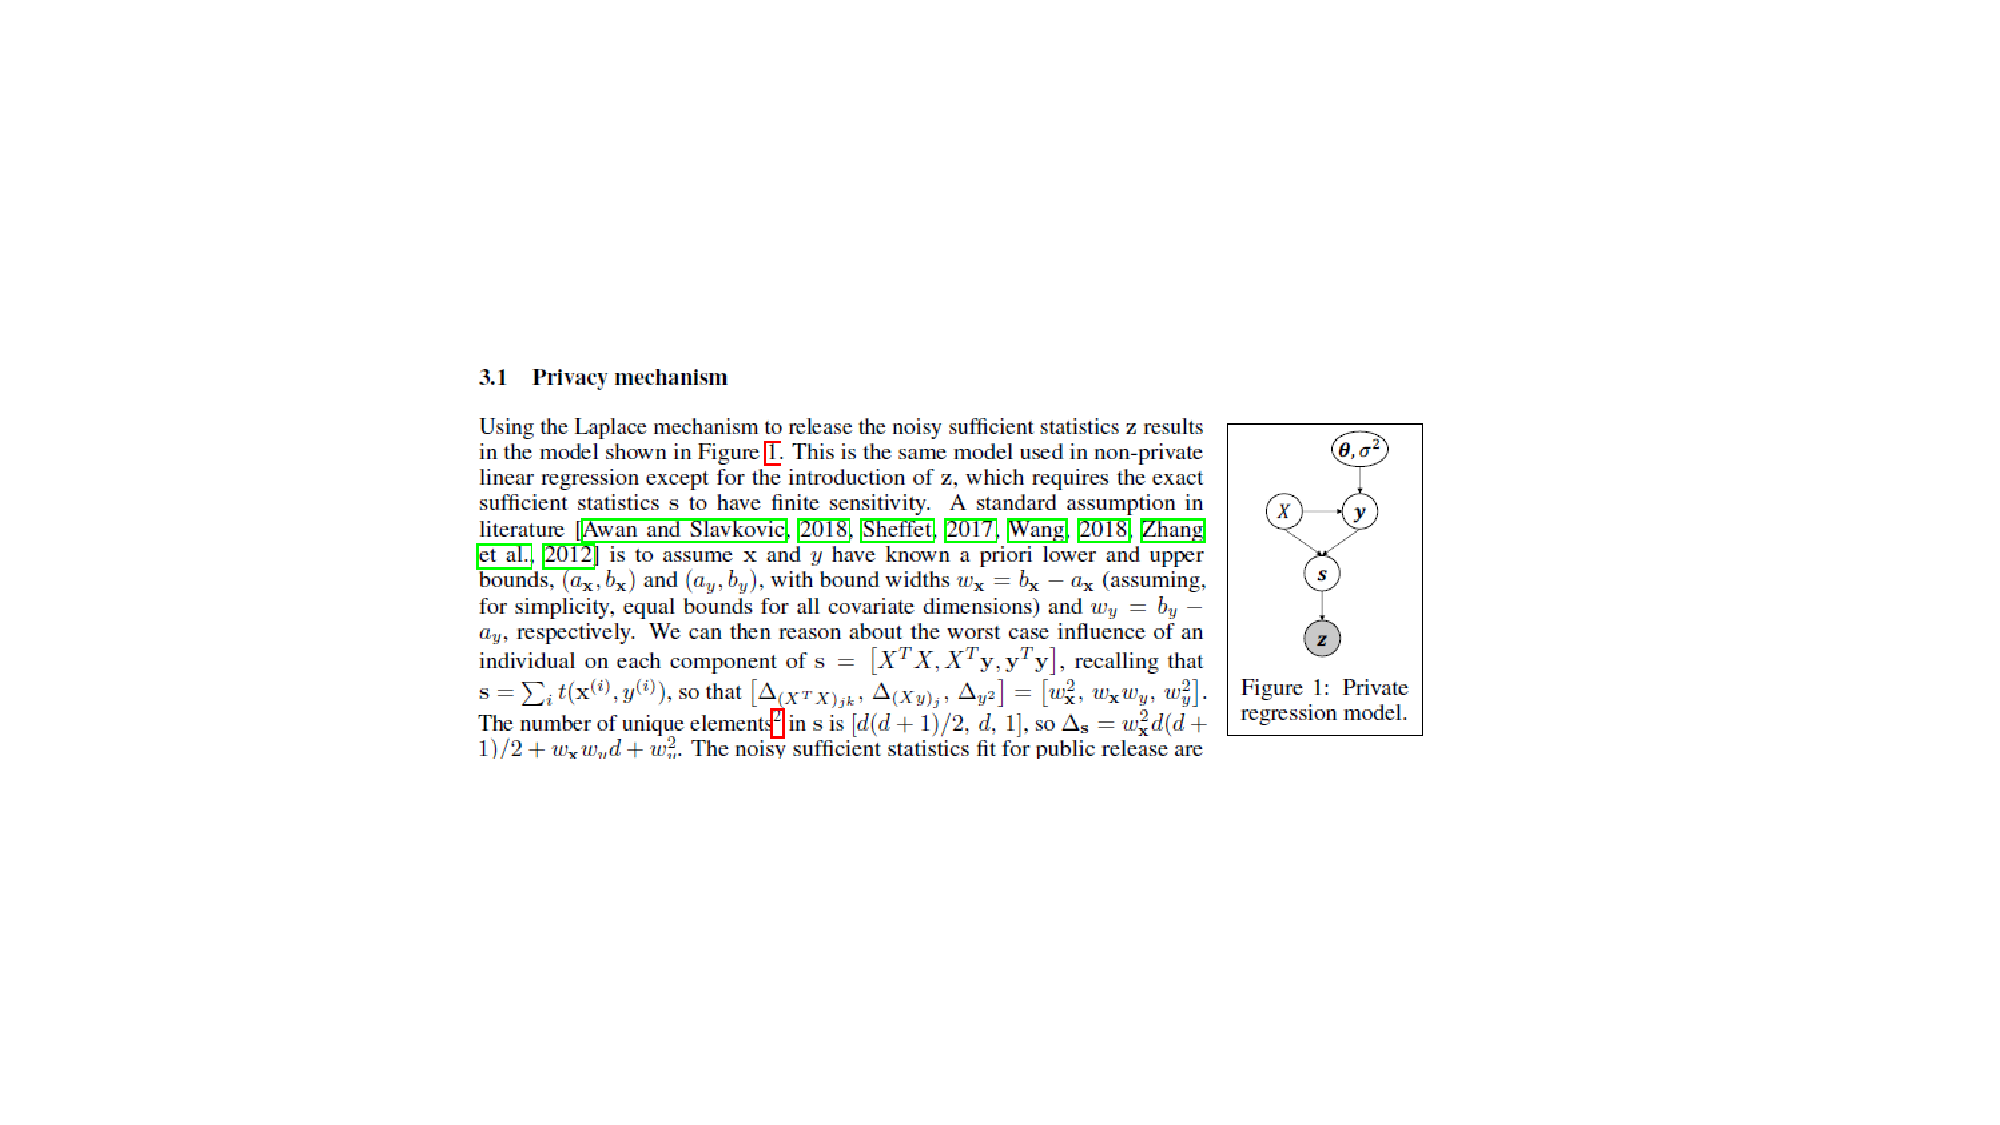
\includegraphics[clip,trim=3in 0in 0in 2in,width=1.5\textwidth]{../figures/testcut.pdf}
  
\end{frame}
%%%%%%%%%%%%%%%%%%%%%%%%%%%%%%%%%%%%%%%%%%%%%%%%%%%%%%%%%%%%%%%%%%%%%%
\begin{titledslide}{Another example}

  \begin{itemize}
  \item An example from a paper on `causal representation learning' \cite{lippe23:_biscuit}
  \end{itemize}

\adjustbox{trim={0\width} {.62\height} {0\width} {0.05\height},clip}%
  {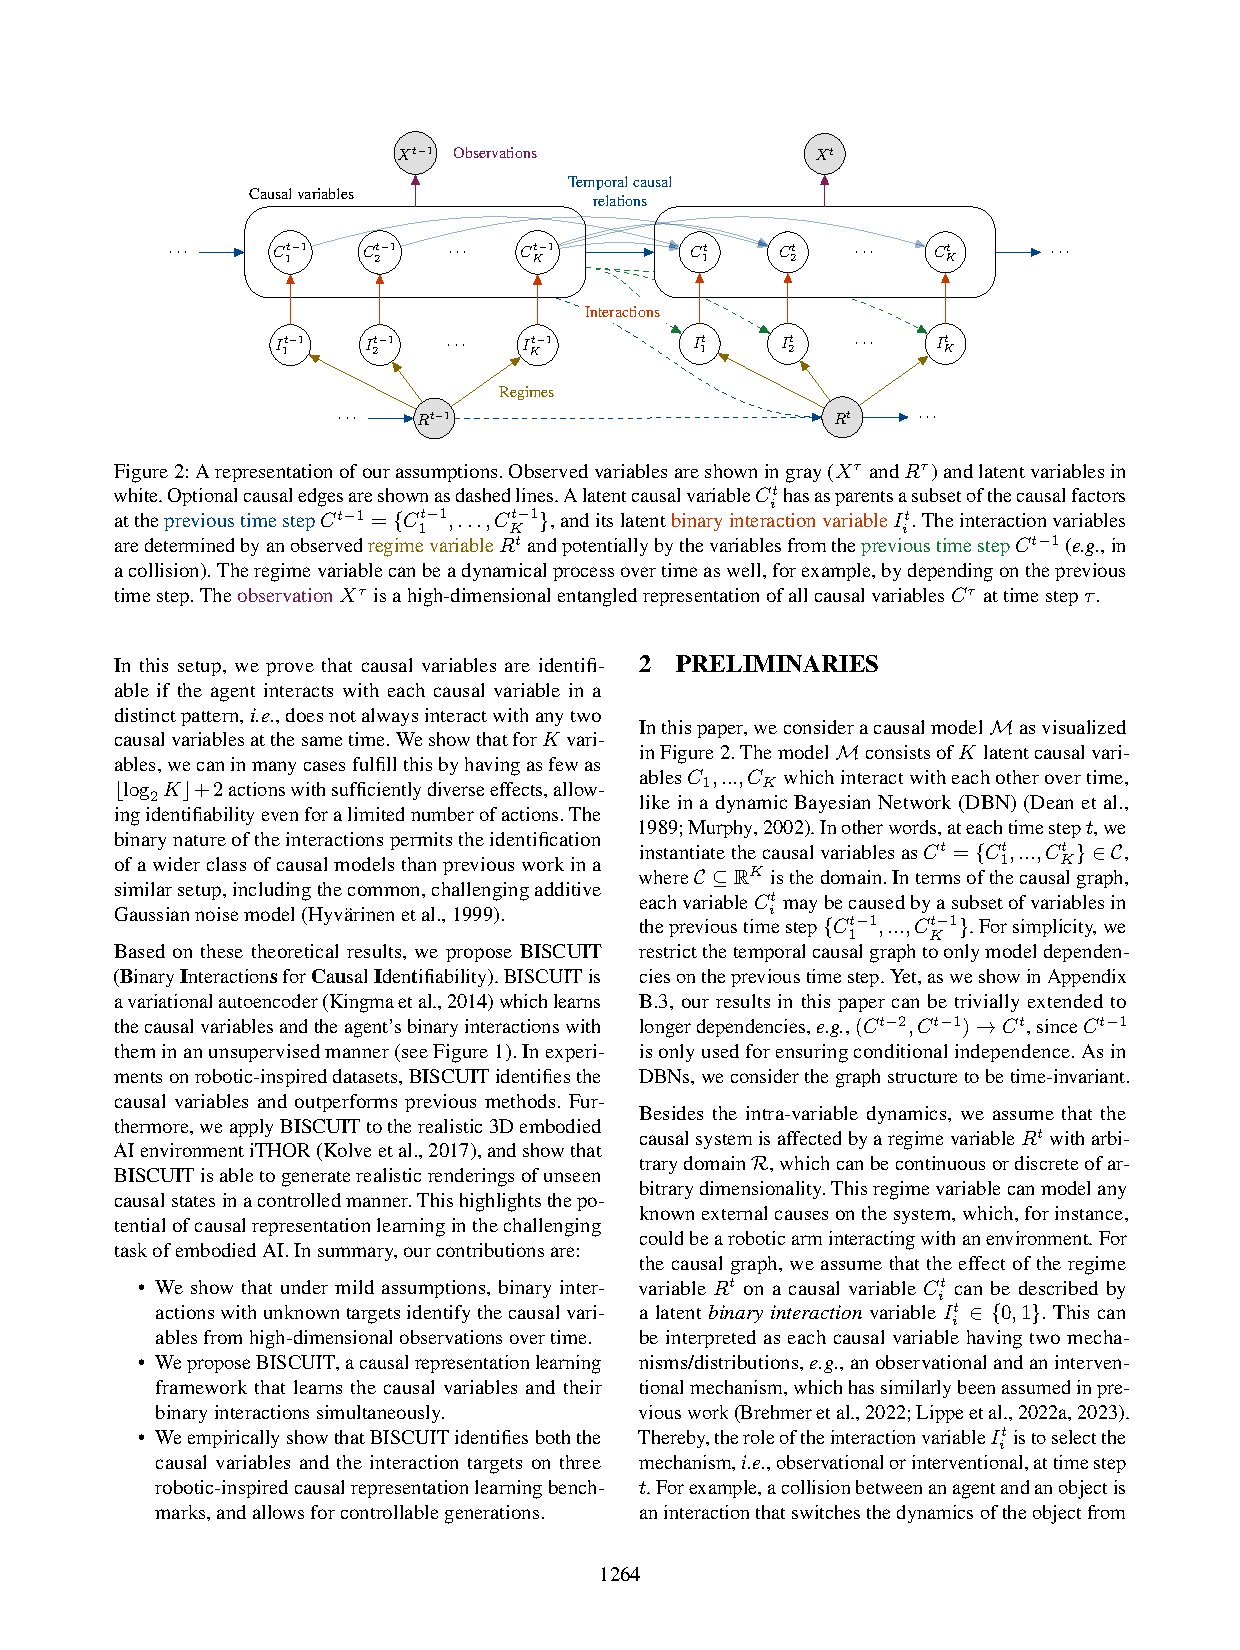
\includegraphics[width=\textwidth]{../figures/lippe-2.pdf}}

  
\end{titledslide}
%%%%%%%%%%%%%%%%%%%%%%%%%%%%%%%%%%%%%%%%%%%%%%%%%%%%%%%%%%%%%%%%%%%%%% 
\begin{frame}
  \frametitle{Naive Bayes}

  \begin{itemize}
  \item In a naive Bayes model for classification
    \cite[p. 380]{bishop06:_patter_recog_machin_learn} the observed
    variables $\xvec = (x_{1}, \dots x_{D})$ are assumed independent
    conditional on the class variable $\mathbf{z}$:
  \end{itemize}
  \begin{equation}
    \label{eq:nbayes}
    P(\xvec,\mathbf{z}) = P(\mathbf{z})P(\xvec|\mathbf{z}) = P(\mathbf{z})\prod_{i=1}^{D}P(x_{i}|\mathbf{z})
  \end{equation}

  \begin{itemize}
\item Let's have a look at a naive Bayes model.
    \cite[p. 163]{pml2Book}.
  \item And a latent variable model \cite[p. 159]{pml2Book}.
  \end{itemize}

\end{frame}


%%%%%%%%%%%%%%%%%%%%%%%%%%%%%%%%%%%%%%%%%%%%%%%%%%%%%%%%%%%%%%%%%%%%%%
% \begin{titledslide}{Naive Bayes}

%     \hspace*{0.5cm}

%   \includegraphics[clip,trim=4.5in 3in 4.5in 2.5in,width=\textwidth]{nbayes.pdf}

%   \[
%     P(\pi,Y,X,\theta) = P(\pi)\left[\prod_{j=1}^{D}P(\theta_{cj})\right]\left\{\prod_{i=1}^{N}\left[P(Y_{i}|\pi) \prod_{j=1}^{D} P(X_{ij}|Y_{i},\theta_{cj})\right]
%   \right\}\]
  
% \end{titledslide}
% %%%%%%%%%%%%%%%%%%%%%%%%%%%%%%%%%%%%%%%%%%%%%%%%%%%%%%%%%%%%%%%%%%%%%%
% \begin{titledslide}{A model with latent variables}
  
%   \includegraphics[clip,trim=4.5in 2.8in 4.5in 2.5in,width=\textwidth]{latent.pdf}

%   \[
%     P(\theta_{x},x,z,\theta_{z}) = P(\theta_{x})P(\theta_{z})\prod_{i=1}^{N}P(z_{i}|\theta_{z})P(x_{i}|z_{i},\theta_{x})
%   \]
  
% \end{titledslide}
%%%%%%%%%%%%%%%%%%%%%%%%%%%%%%%%%%%%%%%%%%%%%%%%%%%%%%%%%%%%%%%%%%%%%%
\begin{frame}
  \frametitle{Hierarchical Linear Regression}

  \href{https://www.pymc.io/projects/docs/en/v3.11.4/pymc-examples/examples/generalized_linear_models/GLM-hierarchical.html}{Here's}
  a nice example of using Bayesian networks to represent different
  approaches to a linear regression problem where there is extra `structure'.

  
\end{frame}
%%%%%%%%%%%%%%%%%%%%%%%%%%%%%%%%%%%%%%%%%%%%%%%%%%%%%%%%%%%%%%%%%%%%%%
\begin{titledslide}{Standard regression (abbreviated)}
  
  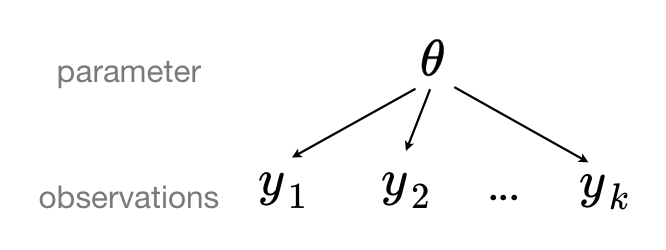
\includegraphics[clip,width=\textwidth]{../figures/linreg1.png}
 
  \[
    P(\theta,y) = P(\theta)\prod_{i=1}^{k}P(y_{i}|\theta)
  \]
\end{titledslide}
%%%%%%%%%%%%%%%%%%%%%%%%%%%%%%%%%%%%%%%%%%%%%%%%%%%%%%%%%%%%%%%%%%%%%
\begin{titledslide}{Separate regressions (abbreviated)}
  
  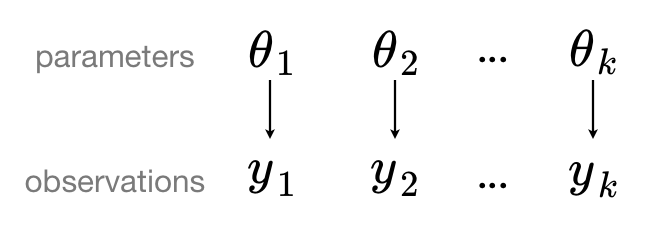
\includegraphics[clip,width=\textwidth]{../figures/separateregressions.png}

    \[
    P(\theta,y) = \prod_{i=1}^{k}P(y_{i}|\theta_{i})P(\theta_{i})
  \]

  
\end{titledslide}
%%%%%%%%%%%%%%%%%%%%%%%%%%%%%%%%%%%%%%%%%%%%%%%%%%%%%%%%%%%%%%%%%%%%%%
\begin{titledslide}{Hierarchical regression (abbreviated)}
  
  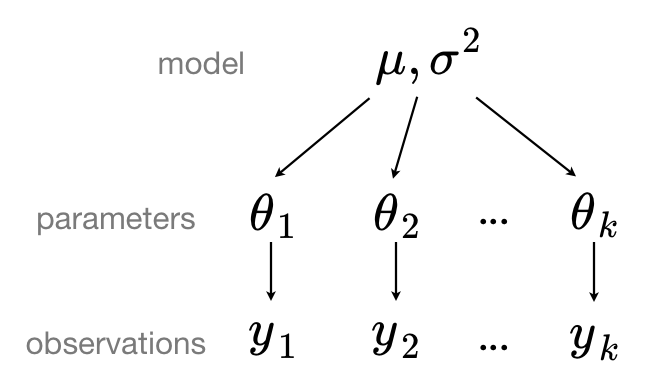
\includegraphics[clip,width=\textwidth]{../figures/hierarchicalregression.png}

      \[
    P(\theta,y,\mu,\sigma^{2}) = P(\mu,\sigma^{2})\prod_{i=1}^{k}P(y_{i}|\theta_{i})P(\theta_{i}|\mu,\sigma^{2})
  \]

  
\end{titledslide}
%%%%%%%%%%%%%%%%%%%%%%%%%%%%%%%%%%%%%%%%%%%%%%%%%%%%%%%%%%%%%%%%%%%%%%
\begin{titledslide}{Conditional independence}

  \begin{itemize}
  \item A random variable $x$ is independent of another random
    variable $y$ \emph{conditional on} a set of random variables $S$
    if and only if:
  \end{itemize}
  \begin{equation}
    \label{eq:condindep}
    P(x,y|S) = P(x|S)P(y|S)
  \end{equation}
  Equivalently:
  \begin{equation}
    \label{eq:condindeptwo}
    P(x|S) = P(x|y,S)
  \end{equation}
  \begin{itemize}
  \item The DAG for a BN encodes conditional independence relations.\pause
  \item Some of the following slides are modified versions of those
    made available by David Barber,
  \item who has written a great (\href{http://web4.cs.ucl.ac.uk/staff/D.Barber/textbook/090310.pdf}{freely available}) book on Bayesian
    machine learning \cite{barber12:_bayes_reason_machin_learn}
  \end{itemize}
\end{titledslide}
%%%%%%%%%%%%%%%%%%%%%%%%%%%%%%%%%%%%%%%%%%%%%%%%%%%%%%%%%%%%%%%%%%%%%%
\begin{frame}[fragile]
  \frametitle{Independence $\ci$ in Bayesian Networks -- Part I}
\vskip0.1cm
All Bayesian networks with three nodes and two links:
\vskip0.1cm
\begin{figure}
\scalebox{0.8}{
\hskip-0.6cm
\begin{subfigure}[b]{0.25\textwidth}
\begin{tikzpicture}%[dgraph]
\node[latent] (x1) at (1,0) {$A$};
\node[latent] (x2) at (3,0) {$B$};
\node[latent] (x3) at (2,-1) {$C$};
\edge{x3} {x1};
\edge{x3} {x2};
%\draw[line width=1.15pt,->](x3)--(x1);\draw[line width=1.15pt,->](x3)--(x2);
\end{tikzpicture}\caption{}
\end{subfigure}
\hskip0.1cm
\begin{subfigure}[b]{0.25\textwidth}
\begin{tikzpicture}%[dgraph]
\node[font=\Large] at (2,1) {$A\ci B \,|\, C$};
\node[latent] (x1) at (1,0) {$A$};
\node[latent] (x2) at (3,0) {$B$};
\node[latent] (x3) at (2,-1) {$C$};
\edge{x1} {x3};
\edge{x3} {x2};
%\draw[line width=1.15pt,->](x1)--(x3);\draw[line width=1.15pt,->](x3)--(x2);
\end{tikzpicture}\caption{}
\end{subfigure}
\hskip0.1cm
\begin{subfigure}[b]{0.25\textwidth}
\begin{tikzpicture}%[dgraph]
\node[latent] (x1) at (1,0) {$A$};
\node[latent] (x2) at (3,0) {$B$};
\node[latent] (x3) at (2,-1) {$C$};
\edge{x3} {x1};
\edge{x2} {x3};
%\draw[line width=1.15pt,->](x3)--(x1);\draw[line width=1.15pt,->](x2)--(x3);
\end{tikzpicture}\caption{}
\end{subfigure}
%\hskip1.2cm
\vrule
\hskip.1cm
%\hskip1.2cm
\begin{subfigure}[b]{0.25\textwidth}
\begin{tikzpicture}%[dgraph]
\node[font=\Large] at (2,1) {$A \,\cancel{\ci}\, B \,|\, C$};
\node[latent] (x1) at (1,0) {$A$};
\node[latent] (x2) at (3,0) {$B$};
\node[latent] (x3) at (2,-1) {$C$};
\edge{x1} {x3};
\edge{x2} {x3};
%\draw[line width=1.15pt,->](x1)--(x3);\draw[line width=1.15pt,->](x2)--(x3);
\end{tikzpicture}\caption{}
\end{subfigure}}
\end{figure}
\vskip0.2cm
\begin{itemize}
\item In (a), (b) and (c), $A$ and $B$ are conditionally independent given $C$.
\vskip0.15cm
\begin{enumerate}
\item[{ (a)}] $p(A,B|C)=\frac{p(A,B,C)}{p(C)}=\frac{p(A|C)p(B|C)p(C)}{p(C)}=p(A|C)p(B|C)$
\vskip0.15cm
\item[{ (b)}] $p(A,B|C)=\frac{p(A)p(C|A)p(B|C)}{p(C)}=\frac{p(A,C)p(B|C)}{p(C)}=p(A|C)p(B|C)$
\vskip0.15cm
\item[{ (c)}] $p(A,B|C)=\frac{p(A|C)p(C|B)p(B)}{p(C)}=\frac{p(A|C)p(B,C)}{p(C)}=p(A|C)p(B|C)$
\end{enumerate}
\vskip0.3cm
\item In (d) the variables $A,B$ are conditionally dependent given
  $C$, $p(A,B|C)\propto p(A,B,C) = p(C|A,B)p(A)p(B)$.
\vskip0.15cm
%\begin{enumerate}
\hskip0.2cm
%\item[] $p(A,B|C)=\frac{p(A,B,C)}{p(C)}=\frac{p(C|A,B)p(A)p(B)}{p(C)}$ \hskip0.1cm in general \hskip0.1cm $\neq p(A|C)p(B|C)$.
%\end{enumerate}
\end{itemize}
\end{frame}
%%%%%%%%%%%%%%%%%%%%%%%%%%%%%%%%%%%%%%%%%%%%%%%%%%%%%%%%%%%%%%%%%%%%%%
%%%%%%%%%%%%%%%%%%%%%%%%%%%%%%%%%%%%%%%%%%%%%%%%%%%%%%%%%%%%%%%%%%%%%%
\begin{frame}[fragile]
  \frametitle{Independence $\ci$ in Bayesian Networks -- Exercises}

\begin{figure}
%\scalebox{0.8}{
\hskip-0.6cm
\begin{subfigure}[b]{0.25\textwidth}
\begin{tikzpicture}%[dgraph]
\node[latent] (x1) at (1,0) {$A$};
\node[latent] (x2) at (3,0) {$B$};
\node[latent] (x3) at (2,-1) {$C$};
\edge{x3} {x1};
\edge{x3} {x2};
%\draw[line width=1.15pt,->](x3)--(x1);\draw[line width=1.15pt,->](x3)--(x2);
\end{tikzpicture}\caption{}
\end{subfigure}
\hskip0.1cm
\begin{subfigure}[b]{0.25\textwidth}
\begin{tikzpicture}%[dgraph]
\node[font=\Large] at (2,1) {$A\ci B \,|\, C$};
\node[latent] (x1) at (1,0) {$A$};
\node[latent] (x2) at (3,0) {$B$};
\node[latent] (x3) at (2,-1) {$C$};
\edge{x1} {x3};
\edge{x3} {x2};
%\draw[line width=1.15pt,->](x1)--(x3);\draw[line width=1.15pt,->](x3)--(x2);
\end{tikzpicture}\caption{}
\end{subfigure}
\hskip0.1cm
\begin{subfigure}[b]{0.25\textwidth}
\begin{tikzpicture}%[dgraph]
\node[latent] (x1) at (1,0) {$A$};
\node[latent] (x2) at (3,0) {$B$};
\node[latent] (x3) at (2,-1) {$C$};
\edge{x3} {x1};
\edge{x2} {x3};
%\draw[line width=1.15pt,->](x3)--(x1);\draw[line width=1.15pt,->](x2)--(x3);
\end{tikzpicture}\caption{}
\end{subfigure}
%\hskip1.2cm
\vrule
\hskip.1cm
%\hskip1.2cm
\begin{subfigure}[b]{0.25\textwidth}
\begin{tikzpicture}%[dgraph]
\node[font=\Large] at (2,1) {$A \,\cancel{\ci}\, B \,|\, C$};
\node[latent] (x1) at (1,0) {$A$};
\node[latent] (x2) at (3,0) {$B$};
\node[latent] (x3) at (2,-1) {$C$};
\edge{x1} {x3};
\edge{x2} {x3};
%\draw[line width=1.15pt,->](x1)--(x3);\draw[line width=1.15pt,->](x2)--(x3);
\end{tikzpicture}\caption{}
\end{subfigure}
\end{figure}%}
\vskip0.2cm
\begin{itemize}
\item Show that in (d), we have $A \ci B$.
\item For each of (a), (b) and (c), assume that each variable is
  binary, and find parameters so that $A \cancel{\ci} B$
\end{itemize}
\end{frame}
%%%%%%%%%%%%%%%%%%%%%%%%%%%%%%%%%%%%%%%%%%%%%%%%%%%%%%%%%%%%%%%%%%%%%%
\begin{frame}[fragile]
  \frametitle{Paths and colliders}

\[
p(A,B,C,D,E)=p(A)p(B)p(C|A,B)p(D|C)p(E|B,C)
\]

  
   \begin{tikzpicture}%[dgraph]
 \node[latent] (x1) at (0,2.1) {$A$};
 \node[latent] (x2) at (2,2.1) {$B$};
 \node[latent] (x3) at (1,1) {$C$};
 \node[latent] (x4) at (-0.2,0.1) {$D$};
 \node[latent] (x5) at (2.5,-0.1) {$E$};
 \edge{x1}  {x3};
 \edge{x2} {x5};
 \edge{x2} {x3};
 \edge{x3} {x4};
 \edge{x3}  {x5};
 \end{tikzpicture}

 \begin{itemize}
 \item A node is a \emph{collider} on some path if both arrows point
   into it on that path.
 \item $C$ is a collider on the path $(A,C,B)$ but is not a
   collider on the path $(A,C,E)$ or on any of the following paths:
   $(A,C,E,B)$, $(D,C,B)$ or $(D,C,E)$. 
 \end{itemize}
 
\end{frame}
%%%%%%%%%%%%%%%%%%%%%%%%%%%%%%%%%%%%%%%%%%%%%%%%%%%%%%%%%%%%%%%%%%%%%%
\begin{frame}[fragile]
  \frametitle{$d$-separation}

  \begin{itemize}
  \item If all paths from node $x$ to node $y$ are \emph{blocked
      given nodes $S$} then $x$ and $y$ are \emph{d-separated} by $S$.
  \item A path is blocked by $S$ if at least one of the following is
    the case:
    \begin{enumerate}
    \item there is a collider on the path that is not in $S$ and none
      of its descendants are in $S$
    \item there is a non-collider on the path that is in $S$.
    \end{enumerate}
  \item If $x$ and $y$ are \emph{d-separated} by $S$ then $x \ci y |
    S$ for any probability distribution which factorises according to
    the DAG.
  \item Let's do some $d$-separation exercises.
  \end{itemize}
\end{frame}
%%%%%%%%%%%%%%%%%%%%%%%%%%%%%%%%%%%%%%%%%%%%%%%%%%%%%%%%%%%%%%%%%%%%%% 
\begin{frame}[fragile]
  \frametitle{Checking for $d$-separation}

   \begin{tikzpicture}%[dgraph]
 \node[latent] (x1) at (0,2.1) {$A$};
 \node[latent] (x2) at (2,2.1) {$B$};
 \node[latent] (x3) at (1,1) {$C$};
 \node[latent] (x4) at (-0.2,0.1) {$D$};
 \node[latent] (x5) at (2.5,-0.1) {$E$};
 \edge{x1}  {x3};
 \edge{x2} {x5};
 \edge{x2} {x3};
 \edge{x3} {x4};
 \edge{x3}  {x5};
\end{tikzpicture}

\vskip1cm

   A path is blocked by $S$ if at least one of the following is
    the case:
    \begin{enumerate}
    \item there is a collider on the path that is not in $S$ and none
      of its descendants are in $S$
    \item there is a non-collider on the path that is in $S$.
    \end{enumerate}

  
\end{frame}
\begin{titledslide}{Hierarchical regression revisited}
  
  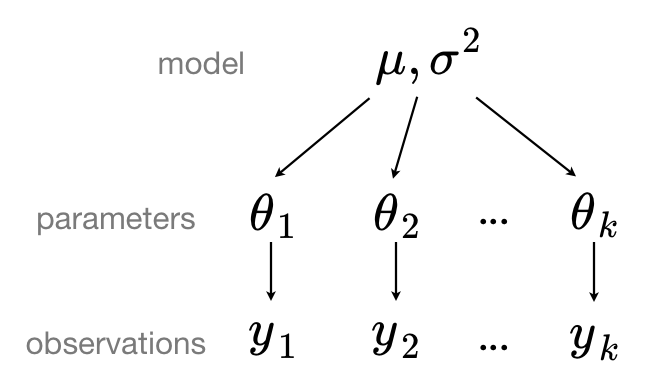
\includegraphics[clip,width=\textwidth]{../figures/hierarchicalregression.png}

      \[
    P(\theta,y,\mu,\sigma^{2}) = P(\mu,\sigma^{2})\prod_{i=1}^{k}P(y_{i}|\theta_{i})P(\theta_{i}|\mu,\sigma^{2})
  \]
\end{titledslide}
\begin{titledslide}{Reading}

  \begin{itemize}
  \item Bishop \S6.1.
  \item Bishop \S7.1 (can skip \S7.1.2). 
  \item Murphy \S17.3 up to \S17.3.8 (skip \S17.3.5 and \S17.3.6)
  \end{itemize}
  
  
\end{titledslide}
%%%%%%%%%%%%%%%%%%%%%%%%%%%%%%%%%%%%%%%%%%%%%%%%%%%%%%%%%%%%%%%%%%%%%%
\begin{titledslide}{Problems and quizzes}

  \begin{itemize}
  \item Do the problems on slide L09: 22/26
    \begin{itemize}
    \item Week~4: Intro to PGMs
    \item Week~4: d-separation
    \end{itemize}
  \end{itemize}
  
\end{titledslide}

\bibliographystyle{alpha}
\bibliography{../ml}

\end{document}
%%%%%%%%%%%%%%%%%%%%%%%%%%%%%%%%%%%%%%%%%%%%%%%%%%%%%%%%%%%%%%%%%%%%%% 

